
\chapter{Schnellere Schnitttests durch Beschleunigungsstrukturen} \label{ch:beschleunigung}

Bisher wurde jeder Primärstrahl mit jedem schnitttestfähigen Objekt in der Szene getestet.
Spätestens mit der Einführung von triangulierten Objekten, die durchaus aus mehreren hunderttausend Dreiecken bestehen können, ist diese Vorgehensweise nicht mehr praktikabel, da so die Laufzeit linear mit der Anzahl an schnitttestfähigen Objekten zunimmt. Mit den folgenden Beschleunigungsstrukturen lässt sich die Anzahl der Schnitttests durch eine obere Grenze von \( O(log(n)) \) beschränken, wobei \( n \) die Anzahl schnitttestfähiger Objekte ist. Der Fokus wird dabei auf die "`bounding interval hierarchy"' (BIH\abk{BIH}{Bounding interval hierarchy}) \cite{wachter2006InsRayTraBouIntHie} gelegt.

\section{Übersicht}

Es existieren bereits verschiedene Ansätze, um die Schnitttests mit der Geometrie zu beschleunigen. Häufig geht es darum, frühzeitig die Objekte auszuschließen, mit denen sicher kein Schnitt vorliegt. Ein erster Schritt, um dies zu erreichen, gelingt durch die Verwendung von Hüllkörpern. Das sind meist sehr einfache Körper wie Kugeln oder Quader, für die ein Schnitttest sehr schnell durchgeführt werden kann. Schneidet ein Strahl den Hüllkörper nicht, so muss auch nicht die umschlossene Geometrie überprüft werden. Schneidet jedoch ein Strahl den Hüllkörper, muss die komplette Geometrie auf Schnitte überprüft werden. Falsch-positive Fälle liegen vor, wenn ein Hüllkörper geschnitten wird, aber kein Schnitt mit der Geometrie gefunden wird. Um solche unnötigen Tests zu vermeiden, sollte der Hüllkörper die Geometrie möglichst eng umschließen.


Ihr volles Potential entfalten Hüllkörper in Kombination mit räumlichen Hierarchien (engl. spatial hierarchy). Dazu gehört z.B. die "`BVH"'\abk{BVH}{Bounding volume hierarchy} (engl. "`bounding volume hierarchy"'). Ziel ist es, die gesamte Geometrie entsprechend ihrer Lage im Raum zu sortieren und in einer Baumstruktur abzulegen. Man beginnt an der Wurzel und erzeugt einen Hüllkörper für die gesamte Geometrie. Nun teilt man die Geometrie anhand eines bestimmten Kriteriums auf, z.B. gleichmäßige Aufteilung der Geometrie auf beide Kindknoten und erzeugt für die aufgeteilte Geometrie kleinere Hüllkörper, die in den Kindknoten gespeichert werden. Dies wird solange fortgesetzt, bis ein Abbruchkriterium erfüllt ist, wie z.B. maximale Tiefe des Baumes oder eine bestimmte Anzahl an Objekten im Knoten, für die keine weitere Teilung durchgeführt wird. Knoten, die eine dieser Bedingungen erfüllen, nennt man Blätter. In ihnen werden Referenzen auf diese Objekte gespeichert. Die Schwierigkeit besteht darin, die Geometrie so aufzuteilen, dass bei der Traversierung des Baumes möglichst nur ein Pfad bearbeitet werden muss. Die Traversierung des Baums beginnt an der Wurzel,
mit dem größten Hüllkörper und wird rekursiv mit Kindknoten fortgesetzt, die ebenfalls vom Strahl geschnitten werden.
 

%Auch bei gleichmäßigen Gittern (engl. uniform grids) kommen Hüllkörper zum Einsatz, werden jedoch nur zur Konstruktion gebraucht.
%Das Gitter besteht aus gleich großen Zellen. 
%
% die aus gleich großen Zellen bestehen. Manche dieser Zellen beinhalten Objekte und andere sind leer. Ein Strahl durchdringt nun nacheinander, die hintereinander liegenden Zellen und führt den Schnitttest nur mit Objekten durch, die sich in der jeweiligen Zelle befinden.

Einen anderen Ansatz verfolgen die "`kd-Trees"'. Hier geht es darum, den Raum so aufzuteilen (engl. space partitioning), dass bei der Traversierung des "`kd-Trees"' möglichst große Raumteile ausgeschlossen werden können und somit die darin befindlichen Objekte nicht getestet werden müssen. Kritisch für die Laufzeit ist hierbei die Wahl der Trennebenen, die den Raum rekursiv in zwei kleinere Bereiche aufteilen. Bei der Traversierung wird getestet, welcher der beiden Raumteile bzw., ob beide Raumteile vom Strahl durchdrungen werden, indem ein Strahl-Ebenen Schnitttest mit der Trennebenen durchgeführt wird. Sobald man einen Raumteil erreicht, der nicht mehr weiter unterteilt ist, werden die darin befindlichen Objekte mit dem Strahl auf Schnitte getestet.


\section{Die "`bounding interval hierarchy"'}

Die Entscheidung auf die "`bounding interval hierarchy"' (BIH) als Beschleunigungsstruktur zu setzen, beruht auf mehreren Gründen.

Für kd-Tree kann vorab nicht entschieden werden, wieviel Speicherplatz im RAM benötigt wird, da Objekte in mehreren Raumteilen referenziert werden können. Denn der Raum kann so geteilt werden, dass ein Objekt in beiden Seiten des geteilten Raumes liegt. Des weiteren birgt das die Problematik von numerischen Instabilitäten und erfordert evt. die Verwendung eines Benachrichtungssystems, um Objekte nicht mehrfach auf Schnitte überprüfen zu müssen.

BVH sind, was die Performance anbelangt, den gut konstruierten kd-Trees unterlegen,
aber dafür recht einfach zu bauen. Der Speicherbedarf kann besser abgeschätzt werden (linear in anzahl der Objekten).
Sie sind numerisch stabiler, da kein Strahl-Ebenen Schnitt, sondern nur min-max Operationen angewendet werden.

Die BIH vereinigt viele der Vorteile beider Methoden, ohne unter deren Nachteile zu leiden.
So sind BIH sehr leicht zu verstehen und zu implementieren, was die Fehleranfälligkeit reduziert. Ihre Konstruktion ähnelt der von BVH, wodurch sie sehr schnell erzeugt werden kann. Damit ist sie für dynamische Szenen oder Echtzeit "`Raytracing"' verwendbar. Die Traversierung verläuft hingegen sehr ähnlich zu der von kd-Trees. Damit ist die BIH nicht nur konkurrenzfähig zu den Traversierungszeiten von kd-Trees, sondern schlägt diese sogar in bestimmten Szenen~\cite{wachter2006InsRayTraBouIntHie}. Jedes Objekt wird exakt einmal in einem Blatt referenziert. Dadurch ist der benötigte Speicherverbrauch vorab berechenbar und es werden keine Benachrichtigungssysteme benötigt.

\subsection{Konstruktion}

Zur Konstruktion der BIH werden "`axis aligned bounding boxes"' (AABB\abk{AABB}{Axis aligned bounding boxes}) benötigt. Das sind quaderförmige Hüllkörper, deren Kanten parallel zu den Achsen des globalen Koordinatensystems verlaufen. Die Repräsentation einer AABB gestaltet sich auf Grund dieser Eigenschaft relativ einfach. Es reicht aus für jede Achse die Ausdehnung der AABB durch einen minimalen und maximalen Wert festzulegen. Die Bezeichner dafür lauten \( min_{x,y,z}, max_{x,y,z} \), wobei das Subskript die entsprechende Achse referenziert.
 
Ein schneller Strahl-AABB Schnitttest (s. Alg.~\ref{alg:strahl_aabb} ) wird in \cite{pharrhumphrey2010Physically} vorgestellt. Dieser liefert, für den Parameter \( t \) aus der Strahlgleichung, die Werte \( t_{min} \) für den nächsten Schnittpunkt und \( t_{max} \) für den entfernteren. Es sei erwähnt, dass der Code so konstruiert wurde, dass er die Besonderheiten der IEEE Spezifikation für Gleitkommazahlen berücksichtigt. So ist die Ausführung des Codes auch dann noch korrekt, wenn eine Komponente \( {\boldsymbol{d}.i } \) des Strahlrichtungsvektor 0 ist und \( d_{inv} \) somit die Werte \( -\infty \) oder \( \infty \) annimmt. Das Gleiche gilt für den Fall, dass der Strahlursprung in einer der Seiten der AABB liegt. Dann kann \( t_{near} \) oder \( t_{far} \) in Zeile 6 und 7 den Wert "`NaN"' annehmen, da \( {\boldsymbol{o}.i } \cdot d_{inv} \) zu "`\( 0 \cdot \pm\infty  \)"' wird. Da Vergleichsoperationen mit "`NaN"' immer "`false"' liefern (außer man vergleicht 2 "`NaN"' miteinander) bleiben \( t_0 \) und \( t_1 \) unverändert.

\begin{algorithm}[H]
    \caption{Schnittest Strahl-AABB}
    \label{alg:strahl_aabb}
    \begin{algorithmic}[1]
        \State \( t_0 \gets -\infty \)
        \State \( t_1 \gets \infty \)\\
        
        \For {\textbf{each} \( i \in \{x,y,z\} \)}
            \State \( d_{inv} \gets 1 / {\boldsymbol{d}.i } \)	\Comment \( \boldsymbol{d}.i  \) \( \equiv \) Komponenten des Strahlrichtungsvektors
            \State \( t_{near} \gets min_i - {\boldsymbol{o}.i } \cdot d_{inv}  \)	\Comment \( {\boldsymbol{o}.i } \) \( \equiv \) Komponenten des Strahlursprungs
            \State \( t_{far} \gets max_i - {\boldsymbol{o}.i } \cdot d_{inv} \)
            
            \If{\( t_{near} > t_{far} \)}
                \State{\( \text{swap}(t_{near}, t_{far}) \)}	\Comment Vertauschen der Werte von \( t_{near} \text{ und } t_{far} \)
            \EndIf
            \If{\( t_{near} > t_0 \)}
                \State \( t_0 \gets t_{near} \)
            \EndIf
            \If{\( t_{far} < t_1 \)}
            \State \( t_1 \gets t_{far} \)
            \EndIf
            \If{\( t_0 > t_1 \)}
                \State\Return{\textbf{false}}
            \EndIf
        \EndFor\\
        
        \State \( t_{min} \gets t_0 \)
        \State \( t_{max} \gets t_1 \)
        \State\Return{\textbf{true}}
       
    \end{algorithmic}
\end{algorithm}

Ziel ist es nun, die Objekte der Szene in einer Baumstruktur abzulegen. Es beginnt damit, eine globale AABB zu erzeugen, die alle Objekte der Szene umfasst. Um die Objekte partitionieren zu können, muss eine Trennebene gefunden werden. Das Konstruktionsverfahren der BIH teilt dazu die globale AABB mittig durch sogenannte Trennebenenkandidaten entlang der längsten Achse auf, wie Abb.~\ref{fig:bih_konstruktion} -a zeigt. Dabei werden nur die Seiten weiter unterteilt, in denen sich auch tatsächlich Objekte befinden. So zeigt Abb.~\ref{fig:bih_konstruktion} -b die final verwendeten Trennebenen, leere Räume sind nicht weiter unterteilt.

\begin{figure}[ht]
    \centering
    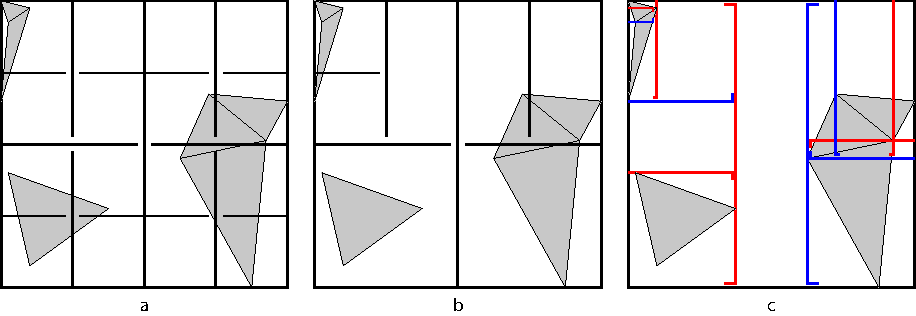
\includegraphics[width=1\textwidth]{./img/beschleunigungsstrukturen/bih_konstruktion.pdf}
    \caption{a) Rekursive Unterteilung der Szene anhand von Trennebenenkandidaten. Die jeweils längste Achse wird mittig durch einen Trennebenenkandidat geteilt. b) Tatsächliche Aufteilung des Raums nach Ablegen der Objekte in Blättern. Leere Räume benötigen keine weitere Unterteilung. c) Rote Klammern zeigen die maximale Ausdehnung der Objekte des linken Kindknoten entlang der geteilten Achse. Blaue Klammern zeigen minimale Ausdehnung der Objekte des rechten Kindknoten. \protect\footnotemark}
    \label{fig:bih_konstruktion}
\end{figure}

\footnotetext{Quelle: \cite{wachter2006InsRayTraBouIntHie} / Seite 5}


Nach Festlegung einer Trennebene wird überprüft, welche Objekte sich links bzw. rechts von der Trennebene befinden. Eine einfache Vorgehensweise besteht darin eine AABB um die zu prüfenden Objekte zu legen und ihren Mittelpunkt zu berechnen. Da die Trennebene immer parallel zu einer der 3 Achsen des globalen Koordinatensystems verläuft, kann die entsprechende Komponente des Mittelpunkts verwendet werden, um die Zuordnung durchzuführen.
Nun wird ein innerer Knoten erzeugt und dieses Schema rekursiv fortgesetzt, bis eine Abbruchbedingung, wie maximale Tiefe des Baumes oder minimale Anzahl zu teilender Objekte erreicht ist. Ist eine Abbruchbedingung erreicht, wird ein Blatt erzeugt und die vom Raumteil des Blattes umschlossenen Objekte im Blatt vermerkt.

Die allgemeine Definition eines Knotens sieht in der Programmiersprache C wie folgt aus und dient zur Erzeugung von inneren Knoten, wie auch Blättern \cite{wachter2006InsRayTraBouIntHie}. Im Folgenden wird erläutert, welche Informationen in inneren Knoten und Blättern gespeichert werden: 

\begin{lstlisting}[language=C,escapeinside=``]
typdef struct
{
  int Index; //LSB: (x=00,y=01,z=10)-Achse oder Blatt(11)
  union
  {
    int   Items;   // Nur Bl`ä`tter
    float Clip[2]; // Nur innere Knoten
  };
} BIH_Node;
\end{lstlisting}


Die beiden niederwertigsten Bit (engl. "`least significant Bit"' LSB \abk{LSB}{Least significant bit}) der Variable "`Index"' werden dazu benutzt, anzuzeigen, ob es sich um ein Blatt handelt, falls nicht, handelt es sich um einen innerer Knoten und die beiden LSB zeigen an, entlang welcher Achse des globalen Koordinatensystems die Unterteilung stattfindet. Die Bedeutung der einzelnen Werte kann der Definition entnommen werden. Die restlichen Bit der Variable "`Index"' werden dazu verwendet, einen Zeiger auf die beiden Kindknoten zu speichern, falls es sich um einen inneren Knoten handelt. Blätter speichern hingegen einen Zeiger auf eine Liste dem Blatt zugeordneter Objekte.
Innere Blätter müssen zudem noch 2 Trennebenen speichern. Dabei handelt es sich nicht um die Trennebenenkandidaten, die zur Partitionierung der Objekte verwendet wurden! Vielmehr wird in Clip[0] die maximale Ausdehnung der Objekte im linken Kindknoten entlang der Koordinatenachse gespeichert und in Clip[1] die minimale Ausdehnung der Objekte im rechten Kindknoten. In Abb.~\ref{fig:bih_konstruktion} -c sind diese Trennebenen durch rote und blaue Klammern gekennzeichnet. Blätter müssen keine Trennebenen speichern, deshalb wird ein "`union"' verwendet, um den ohnehin verbrauchten Speicherplatz für das Speichern der Anzahl im Blatt enthaltener Objekte zu verwenden.


\subsection{Traversierung}

Die Traversierung beginnt damit, dass ein Schnitttest gemäß Algorithmus~\ref*{alg:strahl_aabb} mit der globalen AABB durchgeführt wird. Wenn die globale AABB nicht geschnitten wird, liegt auch kein Schnitt mit der Geometrie vor und die Traversierung endet. Ansonsten erhält man für den Parameter \( t \) der Strahlgleichung die Werte \( t_{min} \) für den nächsten Schnittpunkt und \( t_{max} \) für den entfernteren.
Jetzt wird der Wurzelknoten der BIH zusammen mit \( t_{min} \) und \( t_{max} \) auf einen Stapel (engl. "`stack"') gelegt und die nachfolgenden Anweisungen durchgeführt, bis der Stapel leer ist oder frühzeitig der nächste Schnitt gefunden wurde, wozu die Variable \( t_{Schnitt} \) benötigt wird. Diese wird zu Beginn auf einen sehr großen Wert gesetzt.

\begin{enumerate}
    \item Entnehme den obersten Knoten und die zugehörigen Werte \( t_{min} \) und \( t_{max} \) vom Stapel.
    \item Teste ob \( t_{Schnitt} < t_{min} \), falls ja, fahre mit Anweisung 1. fort. Denn der aktuell zu betrachtende Raumteil ist weiter entfernt als der bisher nächste gefundene Schnittpunkt. Somit können die darin liegenden Objekte unmöglich einen näheren Schnittpunkt liefern.
    \item Teste ob es sich beim aktuellen Knoten um ein Blatt handelt, falls ja, führe Schnitttests mit allen enthaltenen Objekten durch und weise \( t_{Schnitt} \) den minimalen Strahlgleichungsparameter zu. Fahre mit Anweisung 1. fort.
    \item Weise das linke Kind des aktuellen Knotens der Variable \( {KnotenNah } \) und das rechte der Variable \( KnotenFern \) zu. Teste ob die Komponente der Strahlrichtung \( \boldsymbol{d} \), die der Trennebene des aktuellen Knotens entspricht, negativ ist. Falls ja, weise \( KnotenNah \) das rechte und \( KnotenFern \) das linke Kind zu. Somit ist sicher gestellt, dass der Raumteil, der später vom Strahl geschnitten wird, zuerst in den Stapel gelangt und damit nach dem Raumteil betrachtet wird, der zuerst geschnitten wird.
    \item Führe einen Strahl-Ebenen Schnitt mit \( cNah = (\verb|Clip[0]|
    - \boldsymbol{p}.i) * {\boldsymbol{d}.i}^{-1} \) durch, wobei \verb|Clip[0]| die Position der Trennebene des linken Teilraumes beinhaltet (s. Definition BIH\_Node). \( \boldsymbol{p}.i \) und \( \boldsymbol{d}.i \) sind die Komponenten des Strahlursprungs und der Strahlrichtung, wobei \( i \) die Achse ist, auf die sich die Trennebene des aktuellen Knotens bezieht. Berechne \( cFern \) analog, nur mit der Trennebene des rechten Teilraums \verb|Clip[1]| anstelle von \verb|Clip[0]|. Falls \( \boldsymbol{d}.i \)  negativ ist, wurde in Anweisung 4. \( KnotenNah \) und \( KnotenFern \) vertauscht, also tausche auch die Werte von \( cNah \) und \( cFern \), falls \( \boldsymbol{d}.i \) negativ ist.
    \item Teste ob \( cFern \le t_{tmin} \), falls ja, setze \( t_{min} \) auf das Maximum, gebildet aus \( t_{min} \text{ und } cFern\), um den fernen Teilraum weiter einzugrenzen und lege \( KnotenFern \) zusammen mit \( t_{max} \) und dem angepassten \( t_{min} \) auf den Stapel.
    \item Teste ob \( (0 \le cNah) \land (t_{min} \le cNah) \), falls ja, setze \( t_{max} \) auf das Minimum gebildet aus \( t_{max} \) und \( cNah \), um den nahen Teilraum weiter einzugrenzen und lege \( KnotenNah \) zusammen mit \( t_{min} \) und dem angepassten \( t_{max} \) auf den Stapel.
    \item Überprüfe, ob der Stapel leer ist, falls ja, fahre mit Anweisung 9. fort. Ansonsten fahre mit Anweisung 1. fort.
    \item Wenn sich \( t_{Schnitt} \) vom initial zugewiesen Wert unterscheidet, kam ein Schnitt zustande, ansonsten nicht. \( t_{Schnitt} \), verwendet als Strahlgleichungsparameter, liefert dann den nächsten Schnitt. Ende.
    
\end{enumerate}

Ein Detail ist in der beschriebenen Traversierung noch nicht beachtet worden. Und zwar können Strahlen parallel zu den Koordinatenebenen verlaufen, wodurch mindestens eine Komponente der Strahlrichtung \( \boldsymbol{d} \) gleich 0 sein wird. Damit liefert der Schnitttest aus Anweisung 5. die Werte \( \infty \) und \( -\infty \) wegen Division durch 0, bzw. "`NaN"' wenn die Komponente \( \boldsymbol{p}.i \) des Strahlursprungs mit einer der Trennebenenpositionen aus \verb|Clip[0]| oder \verb|Clip[1]| übereinstimmt, wegen der Berechung \( \frac{0}{0} \). Diese Spezialfälle müssen noch gesondert überprüft werden.


\subsection{Geschwindigkeitsmessung}\label{subs:geschwindigkeitsmessung}

Ziel dieses Abschnittes ist es, die Geschwindigkeit der BIH anhand zweier Szenen zu demonstrieren und den Unterschied zur Ausführung des "`Raytracers"' ohne Beschleunigungsstruktur zu zeigen. Gemessen wird die Zeit, die die BIH zur Konstruktion benötigt, sowie die Laufzeit des reinen Renderprozesses, dessen größter Anteil in der Traversierung der BIH besteht. Die Messung findet auf einem "`Intel i5-3570k"' Prozessor statt. Die zu rendernden Szenen besitzen eine Auflösung von \( 800 \times 800 \) Pixel. Jeder Pixel wird anhand eines Primärstrahls durch den Mittelpunkt berechnet.

\begin{minipage}[t]{0.48\textwidth}
    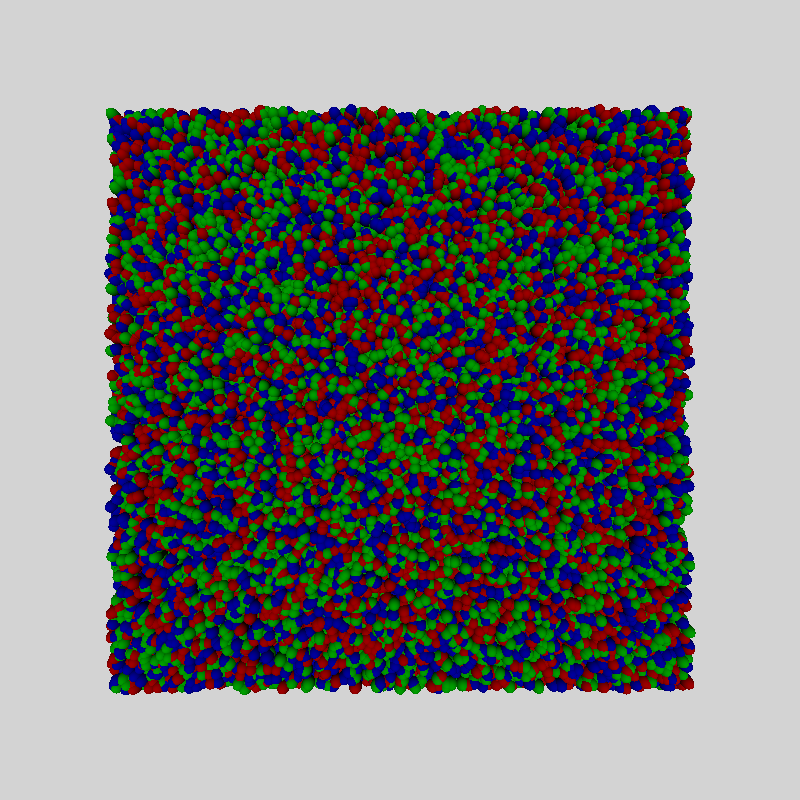
\includegraphics[width=\textwidth]{./img/beschleunigungsstrukturen/1mio_spheres_800x800pxl.png}
    \captionof{figure}{Die Testszene "`Kugeln"' zeigt 1 Million, innerhalb eines Würfels mit der Kantenlänge 9, gleichverteilte Kugeln. Die Auflösung des Bilds beträgt $800 \times 800$ Pixel. }
    \label{fig:1mio_spheres}
\end{minipage}
\begin{minipage}[t]{0.48\textwidth}
    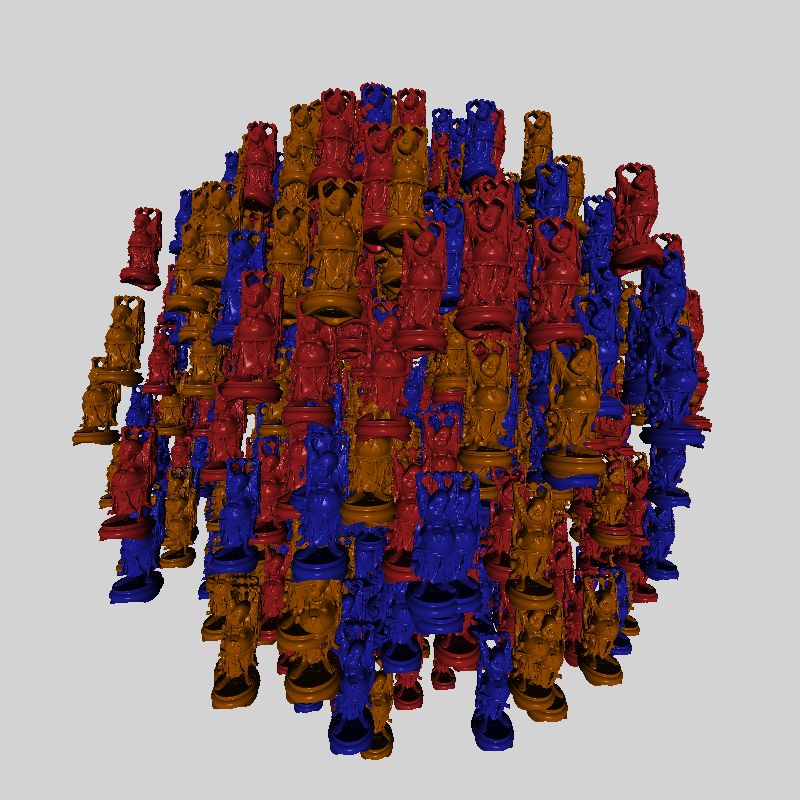
\includegraphics[width=\textwidth]{./img/beschleunigungsstrukturen/1k_buddhas_800x800.png}
    \captionof{figure}{Die Testszene "`Buddhas"' zeigt 1000, innerhalb einer Kugel mit Radius 9, gleichverteilte Stanford Buddhas. Die Auflösung des Bilds beträgt $800 \times 800$ Pixel.}
    \label{fig:1k_buddhas}
\end{minipage}

In der Testszene "`Kugeln"' (s. Abb.~\ref{fig:1mio_spheres} ) werden Kugeln innerhalb eines Würfels mit Kantenlänge 9 gleichverteilt. Es wird die Zeit in Sekunden gemessen, die es dauert die BIH zu erzeugen sowie zu traversieren. Die Erzeugung der BIH findet dabei immer "`single threaded"' statt, wohingegen die Traversierung mit mehreren "`threads"' durchgeführt werden kann. In der Traversierungszeit steckt zudem noch die Zeit, die zur Schattierung der Objekte benötigt wird. Um diese nicht unnötig aufzublähen, wird nur eine Phong-Schattierung verwendet.


 

\begin{figure}[ht]
    \centering
    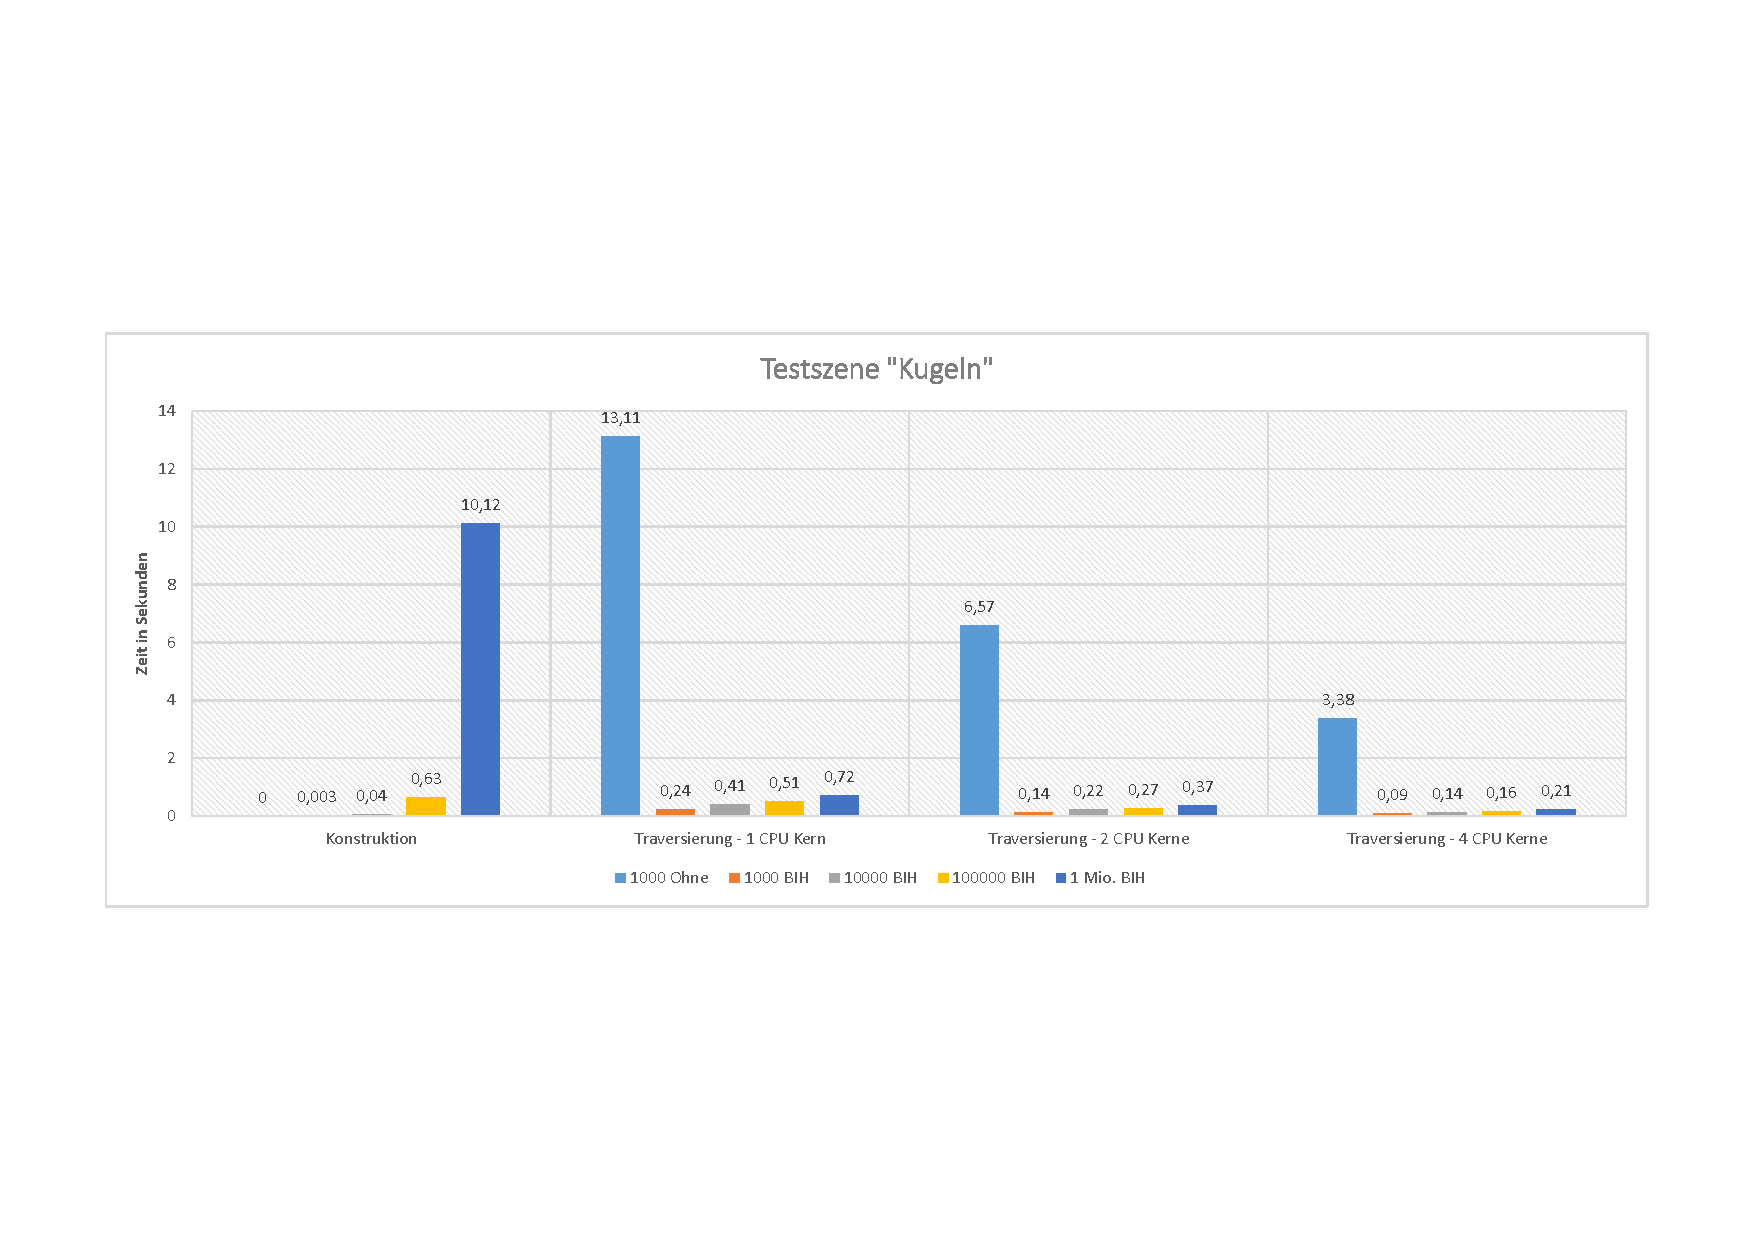
\includegraphics[width=1\textwidth]{./img/beschleunigungsstrukturen/Laufzeiten_Kugelszene.pdf}
    \caption{Zeitmessung in Sekunden der Testszene "`Kugeln"'. Das Diagramm ist unterteilt in Segmente, zur Zeitmessung der Konstruktion sowie der Traversierung der BIH. Die Konstruktion findet immer auf einem CPU Kern statt, wohingegen die Traversierung mit 1, 2 und 4 Kernen durchgeführt wird. Die Balken innerhalb eines Segments stehen für die Anzahl der Objekte in der Szene und zeigen an, ob die BIH verwendet wurde oder nicht ("`Ohne"').  }
    \label{fig:laufzeiten_kugel}
\end{figure}
\begin{figure}[ht]
    \centering
    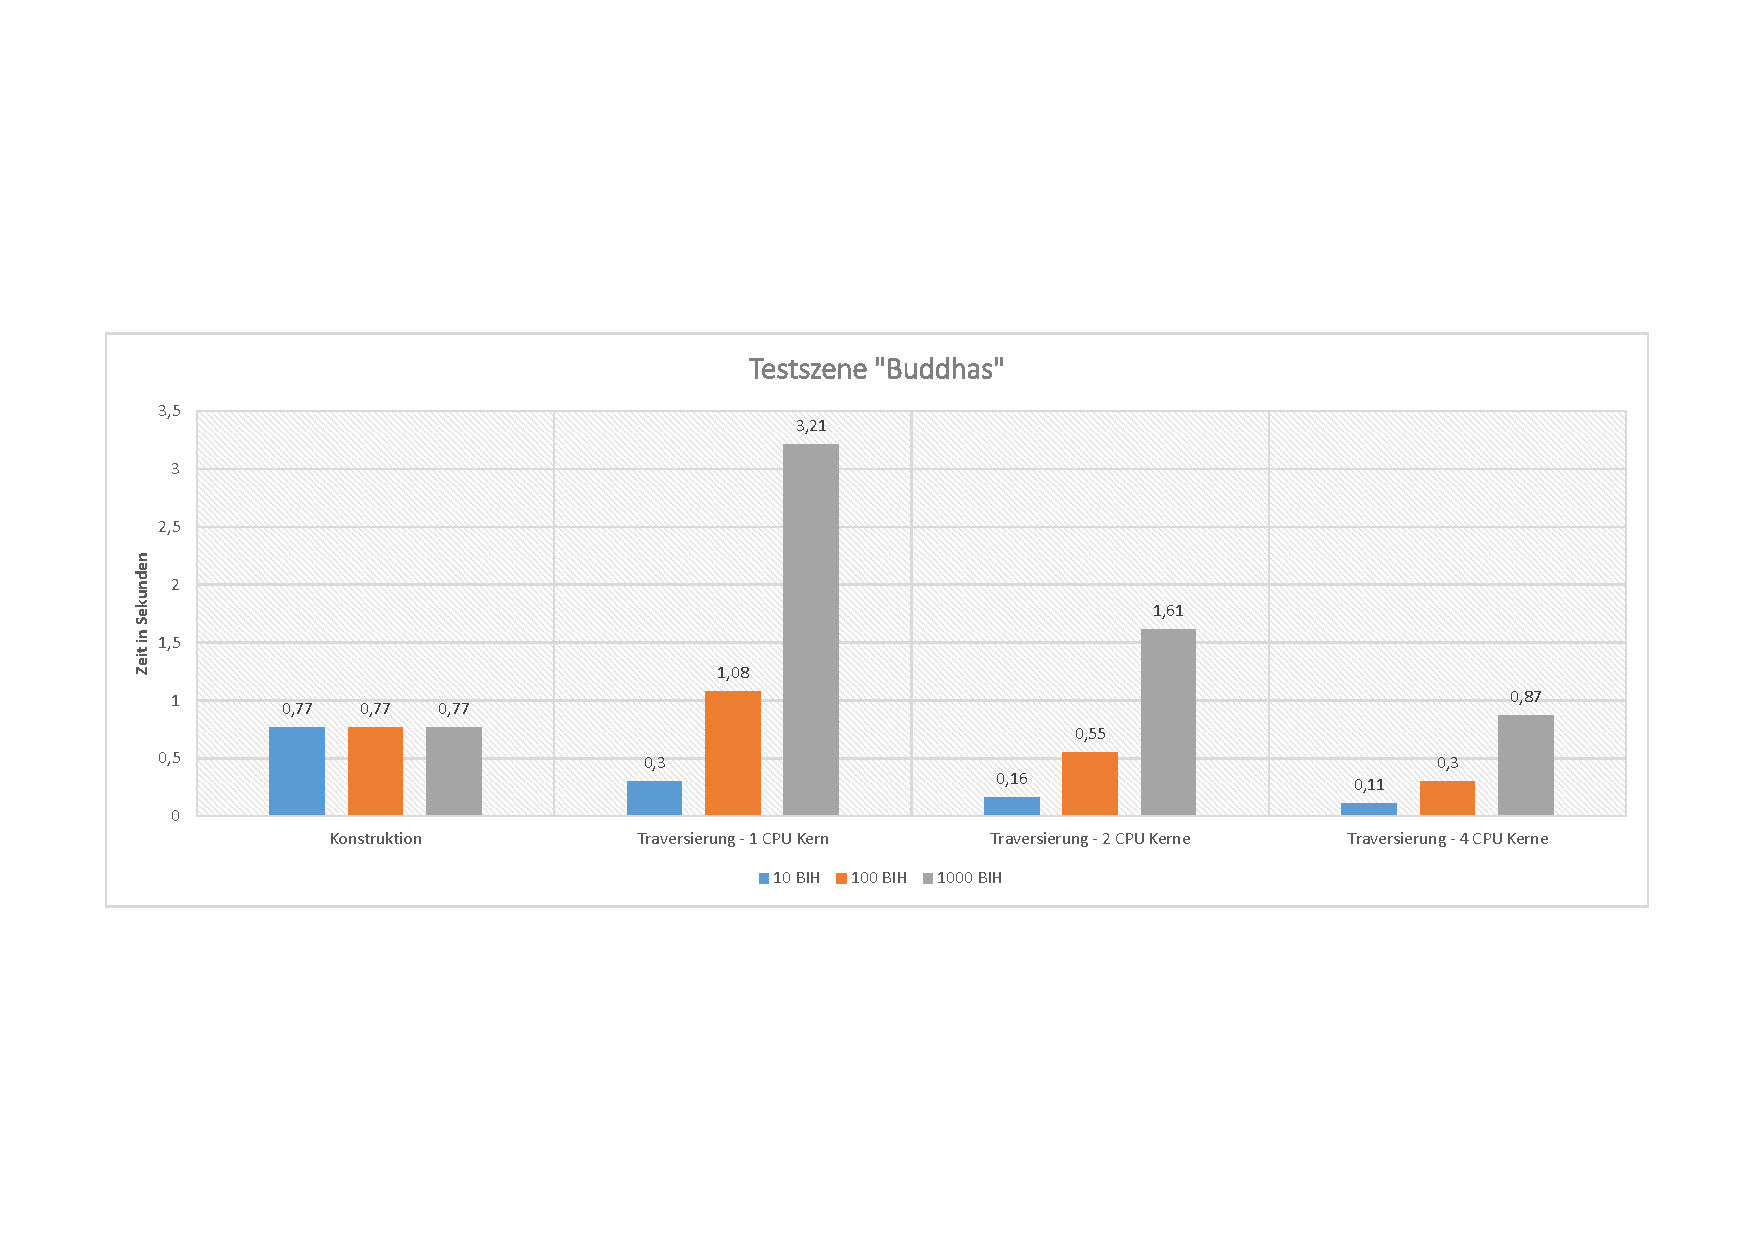
\includegraphics[width=1\textwidth]{./img/beschleunigungsstrukturen/Laufzeiten_Buddhaszene.pdf}
    \caption{Zeitmessung in Sekunden der Testszene "`Buddhas"'. Das Diagramm ist unterteilt in Segmente, zur Zeitmessung der Konstruktion sowie der Traversierung der BIH. Die Konstruktion findet immer auf einem CPU Kern statt, wohingegen die Traversierung mit 1, 2 und 4 Kernen durchgeführt wird. Die Balken innerhalb eines Segments stehen für die Anzahl der Objekte in der Szene. Zum Rendern der Buddhas wurde Instanziierung verwendet, wodurch die Konstruktionszeit gleich bleibt.}
    \label{fig:laufzeiten_buddha}
\end{figure}

Die Messungen aus Abb.~\ref{fig:laufzeiten_kugel} werden für 1000, 10000, 100000 und 1 Million Objekte durchgeführt. Die Diagrammsegmente unterteilen sich in Konstruktionszeit sowie Traversierungszeiten, durchgeführt mit unterschiedlicher Anzahl an "`threads"'. Es zeigt sich bereits bei 1000 Objekten, dass es äußerst unpraktikabel ist jeden Primärstrahl mit jedem Objekt auf Schnitt zu testen. Betrachtet man den Fall, in dem die Konstruktion sowie Traversierung nur auf einem CPU Kern stattfindet, so ist die BIH bei 1 Million Objekte trotz Konstruktionszeit von 10,12 Sekunden und einer Traversierungszeit von 0,72 Sekunden immer noch schneller als der naive Ansatz ohne Beschleunigungsstruktur, der 13,11 Sekunden für 1000 Objekte benötigt.

Für den Stanford Buddha, bestehend aus 100000 Dreiecken, würde das Rendern ohne Beschleunigungsstruktur viel zu lange dauern, weshalb die Zeitmessung nur mit BIH durchgeführt wurde. Die Konstruktionszeiten aus Abb.~\ref{fig:laufzeiten_buddha} zeigen eine Besonderheit, denn sie bleiben konstant, trotz steigender Anzahl Buddhas in der Szene. Dies ist der bereits angesprochenen Instanziierung geschuldet. Es wird nur einmal das Dreiecksnetz des Buddhas geladen und dafür eine BIH erzeugt. Die verschiedenen Instanzen speichern dann eine Referenz auf das Dreiecksnetz und verwenden unterschiedliche Transformationsmatrizen und Materialien.

Ein weiterer Fakt, der aus den Diagrammen hervorgeht, ist die Tatsache, dass die Konstruktionszeit der BIH in \( O(n \cdot log(n)) \) und die Traversierungszeit in \( O(log(n)) \) liegt, wobei \( n \) die Anzahl schnitttestfähiger Objekte ist. Des weiteren zeigt sich, dass "`Raytracer"' prädestiniert dazu sind, parallelisiert zu werden. In der Testszene "`Buddhas"' lässt sich die Traversierungszeit für 1000 Buddhas durch die Verwendung von 4 CPU Kernen fast um Faktor 4 verringern (auf 0,87 Sekunden), im Vergleich zur seriellen Ausführung (3,21 Sekunden) (s.Abb.~\ref{fig:laufzeiten_buddha} ).
 

